\documentclass[14pt]{article}

\usepackage{preamble}
\usepackage{ppc}

\AtBeginDocument{\addtocontents{toc}{\protect\thispagestyle{fancy}}}

%Mise en page en mode fancy : en-têtes et pieds de pages puis définition des en-têtes et pieds de pages%
\pagestyle{fancy}
\cfoot[\thepage]{\thepage}
\begin{document}


%Trait en bas et en haut de la page (entre en-tête et texte et texte et pied de page)%
\renewcommand{\footrulewidth}{0.4pt}
\renewcommand{\headrulewidth}{0.4pt}

\vspace{0cm}              %espace en hauteur (hspace pour la largeur)%
\setstretch{1.4}

%DEBUT DU DOCUMENT%

\import{./}{Front_page.tex}

\clearpage
\thispagestyle{fancy}
\selectlanguage{french}
\tableofcontents
\thispagestyle{fancy}      %Mise en page de la 1ère page en mode fancy%

\clearpage

\section{Choix d'implémentation}

Nous avons implémenté notre solveur en C++.

Le code, et instructions d'utilisation, est accessible via le lien suivant:

 \href{https://github.com/NoemieCERRINA/PPC}{https://github.com/NoemieCERRINA/PPC}

\subsection{Structure des données}

\subsubsection{Structure des contraintes} \label{Structure des contraintes}
Chaque contrainte est modélisée par un objet de classe \texttt{Constraint} qui contient les informations suivantes:
\begin{itemize}
	\item Les indices des variables concernées par la contrainte. Notre solveur ne prenant que des CSP binaires en entrée, il s'agit donc de deux variables entières et ordonnées.
	\item Une liste des paires de valeurs autorisées pour ces variables, sous forme de vecteur de paires d'entiers.
	\item Un dictionnaire de clés où chaque clé correspond à une paire de valeurs autorisées dans le domaine des variables considérées.
\end{itemize}

La liste des paires de valeurs autorisées, implémentée initialement de manière naïve ne permettait la vérification rapide du support d'une variable par une autre. D'où la construction du dictionnaire qui permet quant à lui l'accès en temps constant à la réponse à la question "La paire de variables $x_i$ et $x_j$ peut-elle prendre les valeurs $(v_i,v_j)$ en respectant la contrainte $C(x_i,x_j)$?"

\subsubsection{Structure du CSP}

Afin de résoudre des CSP binaires, nous les avons représenté dans notre solveur à l'aide d'une classe CSP contenant les informations suivantes:

\begin{itemize}
    \item Le nombre de variables du problème sous la forme d'un entier.
    \item Une liste des domaines de chaque variable. Chaque domaine est un entier correspondant aux valeurs autorisées pour chaque variable.
    \item Un vecteur de contraintes, où chaque contrainte est un objet de la classe contraintes décrite dans la section \ref{Structure des contraintes}.
    \item Une matrice des contraintes, où chaque élément en $(i,j)$ est soit un pointeur nul s'il n'existe pas de contrainte entre la variable $x_i$ et $x_j$, soit un pointeur vers la contrainte correspondante. Cette matrice permet l'accès en temps constant à la contrainte entre deux variables $x_i$ et $x_j$ données.
\end{itemize}

\subsection{Représentation fichier}

Afin de standardiser les entrées fournies à notre solveur, on a proposé un format standardisé de fichier d'entrée. Le solveur prend ainsi en entrée un fichier .json dont la structure est décrite ci-dessous:

\begin{verbatim}
	{   "nVar": 2,
	    "Domaines": [{   "vars": [0,1], "values": [0,1]    }],
	    "Constraints": [{   "vars": [[1,0]], "allowed": [[1,1]]    }]}
\end{verbatim}

C'est une description en extension des contraintes binaires de notre CSP, dans laquelle on s'autorise toutefois à réunir les variables qui possèdent les mêmes domaines, ainsi que les couples de variables possédant les mêmes contraintes. Une telle description en extension du problème atteint rapidement ses limites en terme de taille mémoire. Ci-dessous le nombre d'octets nécessaire pour représenter n-queens pour différentes valeurs de n.

\begin{longtable}{|c|c|}
	\hline
	$n$ & Taille mémoire (Mo) \\
	\hline
	\endfirsthead

	$n$ & Taille mémoire (Mo) \\
	\hline
	\endhead

	\hline
	\endfoot

	\hline
	\endlastfoot

	10  & 0.1                 \\
	25  & 1.2                 \\
	50  & 22.2                \\
	100 & 377.2               \\
\end{longtable}

Lorsqu'on double la valeur de n, on augmente la taille mémoire par un facteur 20 environ. Il devient rapidement déraisonnable de souhaiter représenter de tels problèmes en extension pour de plus grande valeurs de n. En pratique on se limitera à n=100 pour les instances de n-reines considérées plus bas. On constatera qu'à priori notre solveur pourrait résoudre des instances de n-reines de taille plus grande, mais qu'alors le temps de chargement des données en mémoire devient très important.

\subsection{Implémentation d'algorithmes} \label{Implémentation d'algorithmes}

Parmi les méthodes présentées dans le cours, on a choisi d'implémenter les suivantes :
\begin{itemize}
	\item Backtrack \textbf{[Bck]} - On vérifie simplement que la nouvelle variable instanciée ne viole aucune des contraintes portant sur des variables déjà instanciées.
	\item Forward Checking \textbf{[FC]} - On met à jour le domaine de toutes les variables à partir de la nouvelle variable instanciée.
	\item Maintain Arc Consistency \textbf{[MAC3]} et \textbf{[MAC4]} - On met à jour le domaine de toutes les variables à partir de la nouvelle variable instanciée, puis on propage jusqu'à ce que toutes les valeurs soient supportées.
\end{itemize}

Dans chacune des méthodes présentées ci-dessus, on explore l'arbre d'instanciation des variables en profondeur. C'est à dire qu'une fois qu'on a assigné une valeur à une variable, on explore toutes les possibilités pour cette assignation partielle avant de potentiellement assigner une autre valeur à cette variable. Toutes les méthodes sont implémentées de manière récursive, et suivent les étapes suivantes :
\begin{enumerate}
	\item \textbf{Mise à jour des domaines} - Via un des algorithmes présentés ci-dessus.
	\item \textbf{Backtrack 1} - Vérifier si un des domaines devient vide suite à l'instanciation de la dernière variable.
	\item \textbf{Choix d'une variable à instancier} - Différentes heuristiques de choix de variable possibles.
	\item \textbf{Itération sur les valeurs} - Retourner VRAI si on obtient une solution réalisable pour une des valeurs.
	\item \textbf{Backtrack 2} - Retourner FAUX si aucune des valeurs ne permet d'aboutir à une solution réalisable.
\end{enumerate}

Au vu du nombre important d'appels récursif de la méthode de résolution, la question de la représentation mémoire des domaines à chaque étape est primordiale. Pour éviter de copier l'ensemble des domaines en chaque nœud de l'arbre, nous avons, comme suggéré durant le cours, choisi de conserver, pour chaque variable, un seul vecteur global du domaine en mémoire, et de passer comme paramètre de la fonction l'indice du dernier élément $last\_elt$ du domaine dans ce vecteur. Lorsqu'on retire un élément du domaine, on échange en pratique cet élément avec l'élément d'indice $last\_elt$, puis on diminue la valeur de $last\_elt$ de 1. 

\clearpage

\section{Évaluation du solveur}

\subsection{Évaluation du choix de la méthode de résolution}

On évalue ici chacune des méthodes présentées dans la section \ref{Implémentation d'algorithmes}. On compare les performances avec celles du solveur \href{https://developers.google.com/optimization/cp/cp_solver?hl=fr}{[CP-SAT] de Google OR-Tools}. Les variables sont ici choisies dans l'ordre dans lesquelles elles apparaissent.

\subsubsection{Évaluation sur n-reines}

On présente ci-dessous une évaluation des performances de notre solveur quant au temps de résolution nécessaire pour exhiber une solution du problème n-reines. On utilise la formulation compacte (celles ayant le minimum de variables) du problème n-reines :

Chaque variable $x_i$ correspond à la position de la reine sur la ligne $i$, et son domaine est $\{0, 1, \dots, n-1\}$.
\[
	\begin{cases}
		x_i \neq x_j,             & \forall i \neq j \quad \text{(pas deux reines sur la même colonne)}   \\
		|x_i - x_j| \neq |i - j|, & \forall i \neq j \quad \text{(pas deux reines sur la même diagonale)}
	\end{cases}
\]

Le graphique ci-dessous montre le nombre d'instances de n-queens, $n \in \{15,\dots,35\}$, résolues en moins de 30 secondes par chacune des méthodes ci-dessus. Il est important de noter ici que l'on ne considère pas le temps, non-négligeable, nécessaire pour charger l'instance en mémoire.

\begin{figure}[H]
	\centering
	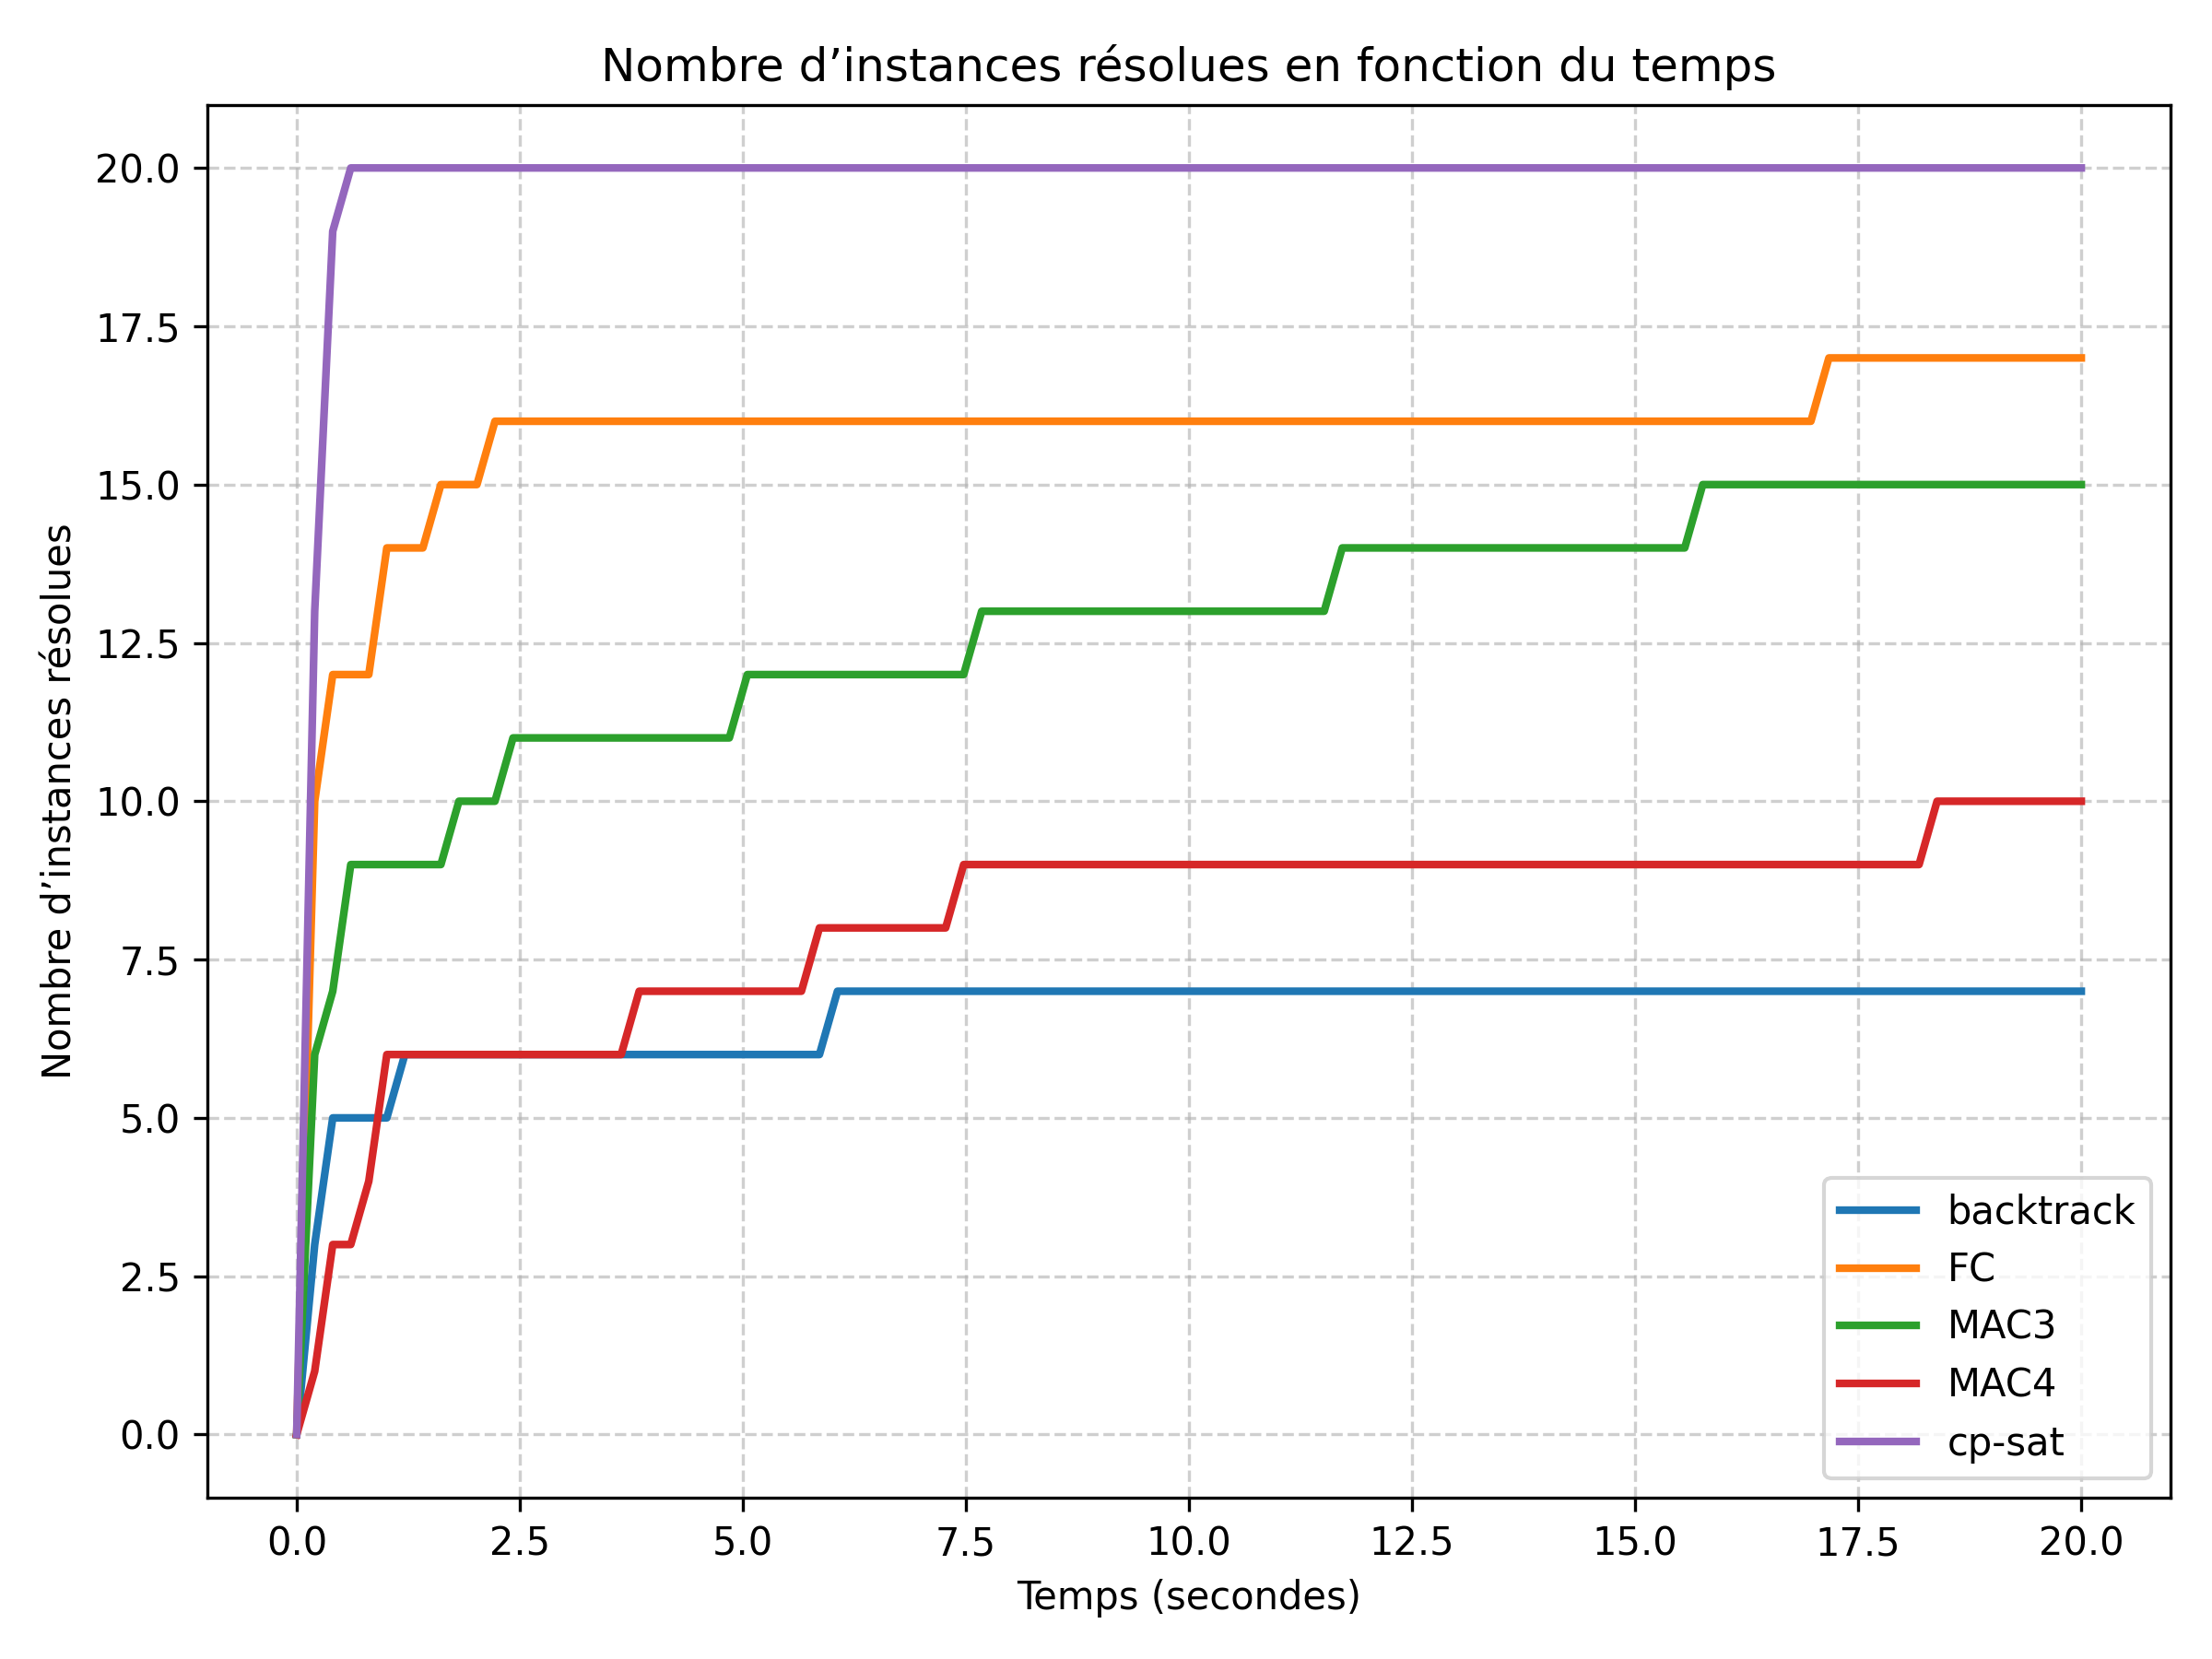
\includegraphics[width=0.8\textwidth]{Images/n-queens1.png}
	\caption{Nombre d'instances de n-queens que l'on peut résoudre en moins de t secondes.}
	\label{fig:n-queens1}
\end{figure}

On constate sur ce graphique, que pour ce type de problème, l'algorithme [FC] est le plus efficace. De manière, peut-être, surprenante, l'algorithme [MAC4] a de moins bonnes performances que [MAC3], alors que [MAC4] a une complexité théorique normalement meilleure. Il se peut que [MAC4] fonctionne mieux que [MAC3] sur de plus grandes instances.

On présente dans le tableau suivant la plus grande instance de n-queens résolue en moins de 30 secondes, pour des valeurs de $n \in \{15,\dots,35\}$.

\begin{longtable}{|c|c|}
	\hline
	Méthode & Plus grande instance résolue \\
	\hline
	\endfirsthead

	Méthode & Plus grande instance résolue \\
	\hline
	\endhead

	\hline
	\endfoot

	\hline
	\endlastfoot

	Bck     & 21                           \\
	MAC4    & 25                           \\
	MAC3    & 30                           \\
	FC      & 31                           \\
	CP-SAT  & 35                           \\
\end{longtable}

\subsubsection{Évaluation sur le problème de k-coloriage}

On présente ci-dessous le temps de résolution nécessaire à l'obtention d'une solution pour des problèmes de k-coloriage, choisis par ordre de difficulté croissante. On considère un sous-ensemble des problèmes disponibles à l'adresse \href{https://mat.tepper.cmu.edu/COLOR/instances.html}{https://mat.tepper.cmu.edu/COLOR/instances.html}.\\

Pour représenter une instance de $k$-coloriage en extension, on autorise, pour chaque arête $(x_1,x_2)$ du graphe, tous les couples de valeurs $(v_1,v_2)$ avec $v_1 \neq v_2 \in \{0,1,\dots,k-1\}$.

Le graphique ci-dessous montre le nombre d'instances de k-coloriage résolues en moins de 30 secondes par chacune des méthodes mentionnées. Comparé au problème n-reines, les instances de k-coloriage considérées se chargent toutes rapidement en mémoire.

\begin{figure}[H]
	\centering
	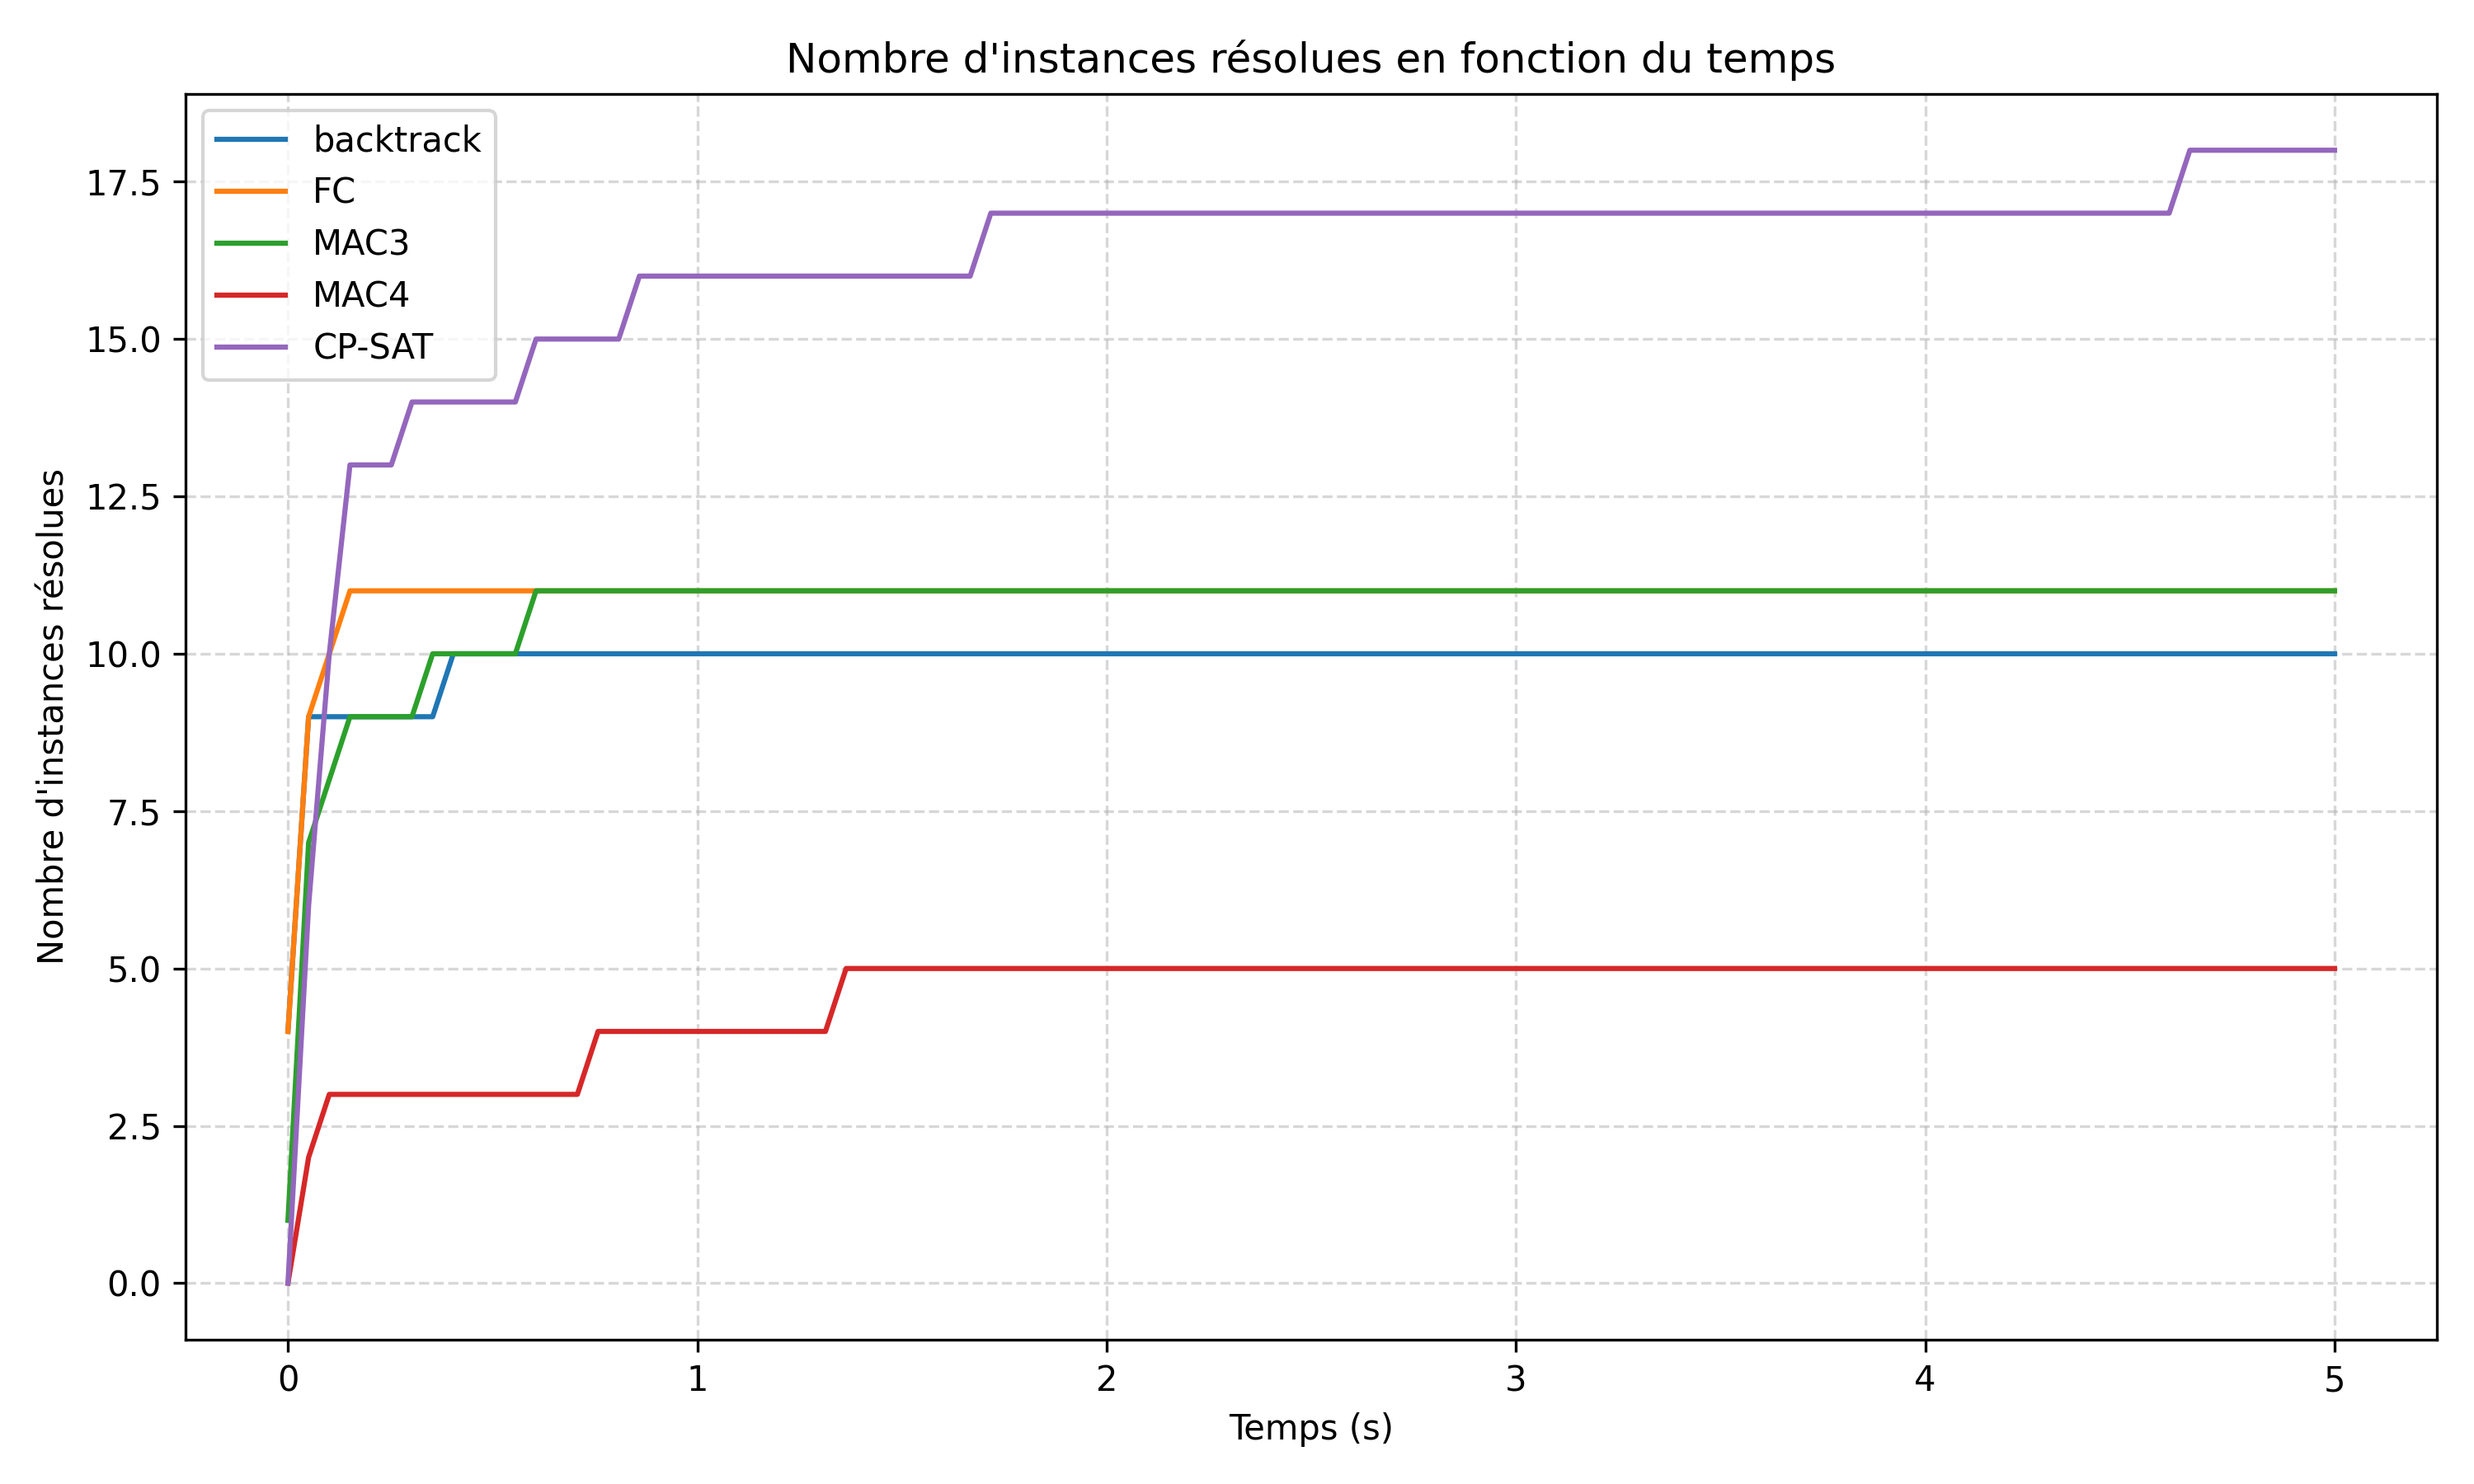
\includegraphics[width=0.8\textwidth]{Images/coloring1.png}
	\caption{Nombre d'instances de k-coloriage que l'on peut résoudre en moins de t secondes.}
	\label{fig:coloring1}
\end{figure}

Sur l'ensemble des instances considérées, la méthode [MAC4] est à nouveau celle qui a les plus mauvaises performances, et [FC] celle qui a les meilleures performances. Une fois encore, le solveur [CP-SAT] a de bien meilleures performances, mais échoue néanmoins à résoudre les deux instances les plus difficiles en moins de 30 secondes.

\subsection{[Approfondissement] Évaluation du choix de sélection de variable}

Dans chacune de nos méthodes de résolution, nous avons employé différentes heuristiques de choix de variables à instancier à chaque étape. Ces méthodes influent fortement sur l'efficacité de l'algorithme.

\subsubsection{Présentation des heuristiques implémentées}

%TODO%
Quatre méthodes de choix de variables ont été implémentées dans notre solveur:
\begin{itemize}
	\item \textbf{h0} - Ordre d'entrée - L'ordre initial dans lequel les variables sont données au solveur. Ce choix par défaut ne signifie quelque chose que si l'ordre donné initialement a un sens vis-à-vis du problème.
	\item \textbf{h1} - Plus petit domaine - A chaque étape, la variable avec le plus petit domaine est choisie.
	\item \textbf{h2} - Plus grand domaine - A chaque étape, la variable avec le plus grand domaine est choisie.
	\item \textbf{h3} - Au hasard - A chaque étape, une variable parmi les variables restantes est choisie au hasard avec une probabilité uniforme sur l'ensemble des variables restantes.
\end{itemize}


\subsubsection{Évaluation sur n-reines}

Évaluons nos différentes heuristiques uniquement sur les méthodes [FC] et [MAC4] qui étaient nos méthodes les plus efficaces de résolution et comparons avec les performances du solveur [CP-SAT] comme dans la partie précédente.

Nous observons sur la figure \ref{fig:n-queens-h1} que sur le problème des n-reines, l'heuristique de choix influe fortement sur la performance de nos algorithmes. [FC] demeure significativement plus performant que [MAC] lorsque la même heuristique de choix est appliquée. Cependant un mauvais choix de variable peut pénaliser un algorithme supposé plus efficace comme le montre la mauvaise performance de [FC] avec l'heuristique de choix du plus grand domaine (h2).

\begin{figure}[H]
	\centering
	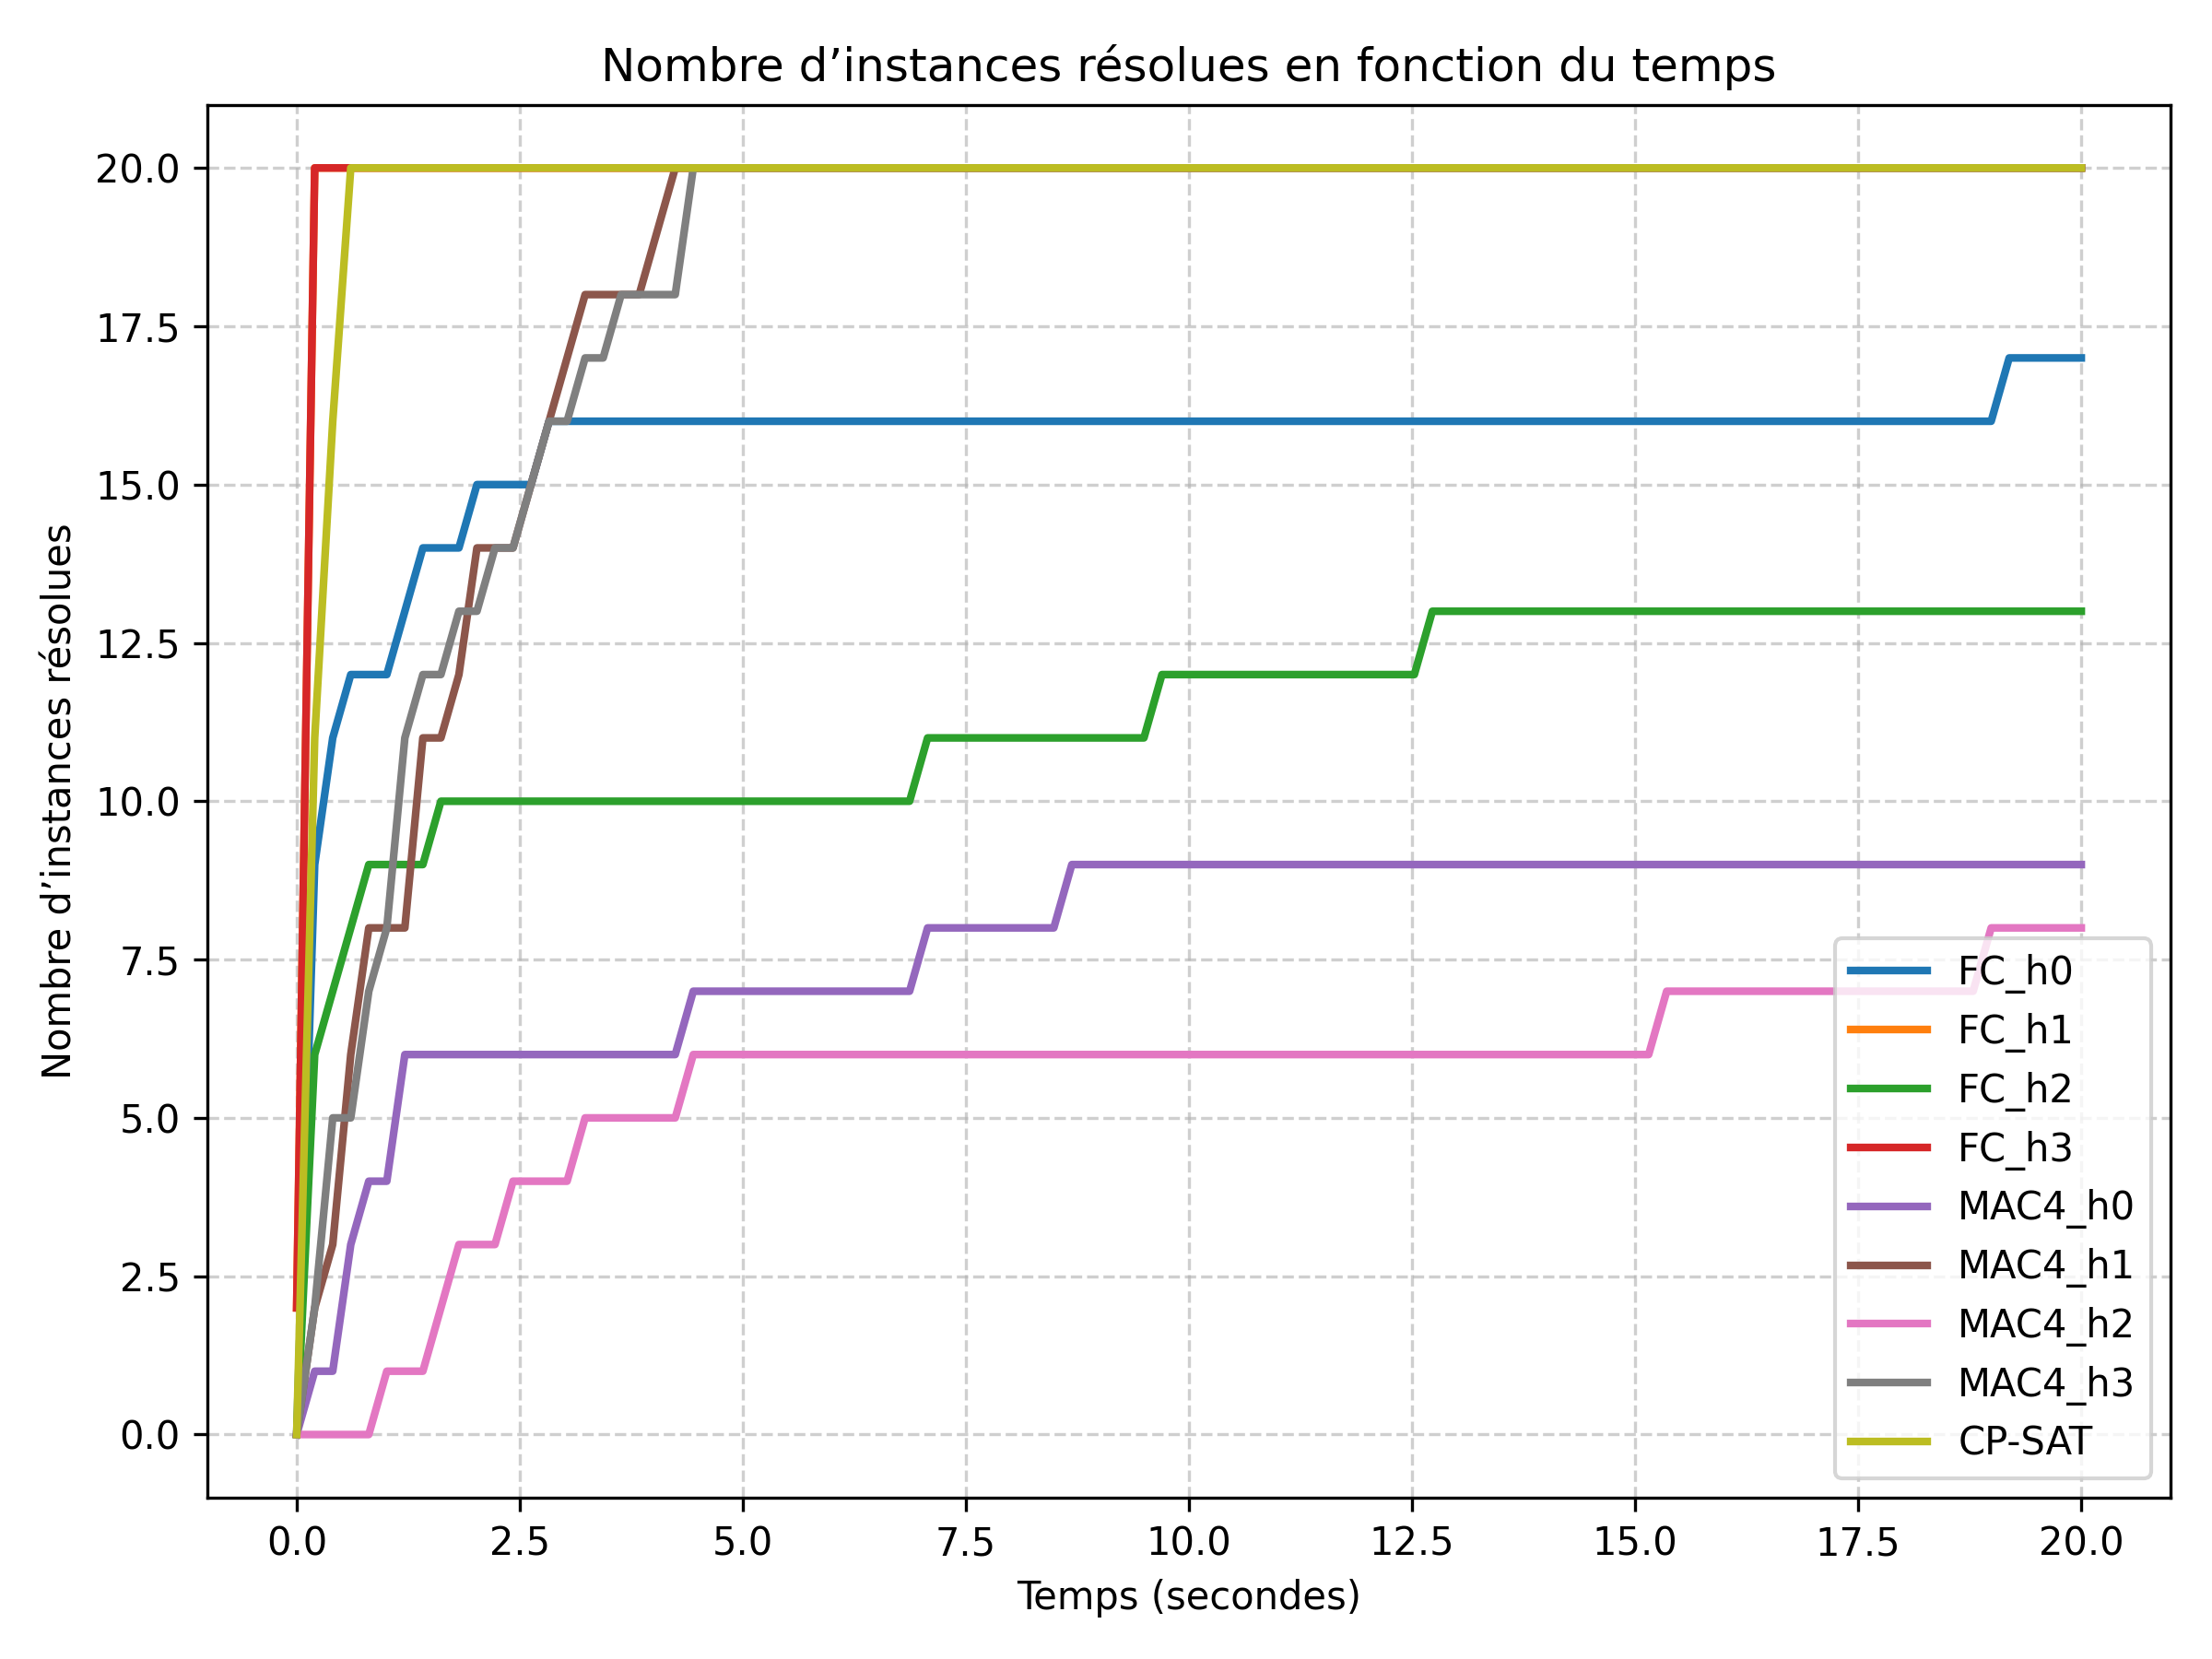
\includegraphics[width=0.77\textwidth]{Images/n-queens-h-MAC-FC.png}
	\caption{Nombre d'instances de n-queens résolues par [FC] et [MAC4] en fonction de l'heuristique de choix}
	\label{fig:n-queens-h1}
\end{figure}

\begin{figure}[H]
	\centering
	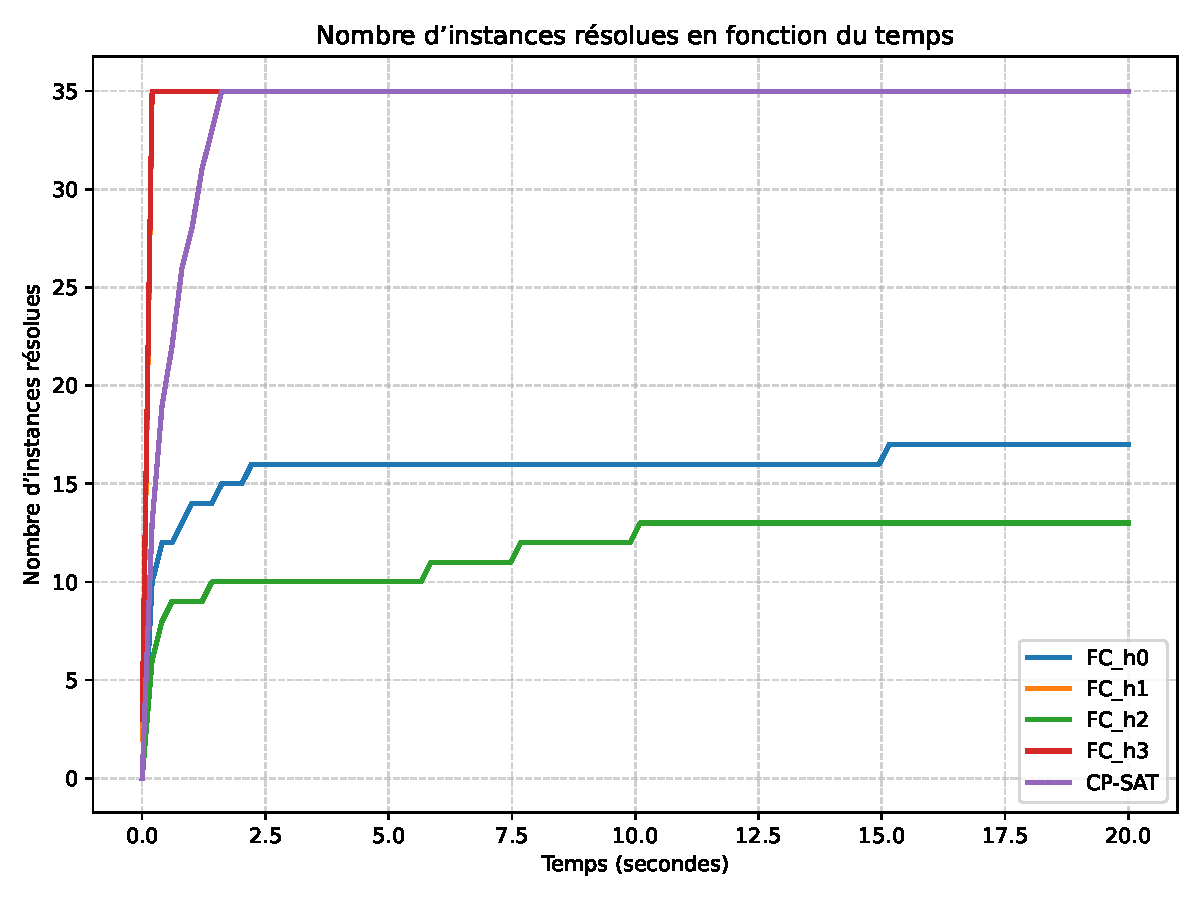
\includegraphics[width=0.8\textwidth]{Images/n-queens-h-FC.pdf}
	\caption{Nombre d'instances de n-queens résolues par [FC] en fonction de l'heuristique de choix}
	\label{fig:n-queens-h2}
\end{figure}

Si nous nous intéressons maintenant uniquement à la comparaison des heuristiques appliquées à [FC] (figure \ref{fig:n-queens-h2}) sur des instances de $n \in 15,...,50$ pour tenter de départager les heuristiques les plus efficaces, nous confirmons la tendance suivante:

\begin{itemize}
	\item La pire heuristique est la \textbf{h2}, qui sélectionne les variables au plus grand domaine à chaque étape, suivie de l'heuristique \textbf{h0} prenant les variables dans l'ordre de départ, ici celle des colonnes de 1 à n.
	\item Nos meilleures heuristiques de choix sont la \textbf{h1}, qui prend la variable au plus petit domaine et la \textbf{h3} qui sélectionne les variables au hasard. Elles rivalisent d'ailleurs avec le solveur [CP-SAT] sur ce problème particulier.
\end{itemize}


\subsubsection{Évaluation sur le problème de k-coloriage}

Evaluons nos différentes heuristiques uniquement sur les méthodes [FC] et [MAC4] qui étaient nos méthodes les plus efficaces de résolution.

Le solveur [CP-SAT] résout l'intégralité de nos instances en moins d'un dixième de seconde donc il serait vain de s'y comparer. Nous observons qu'une grande marge de progression demeure pour que notre solveur soit près d'être compétitif.

\begin{figure}[H]
	\centering
	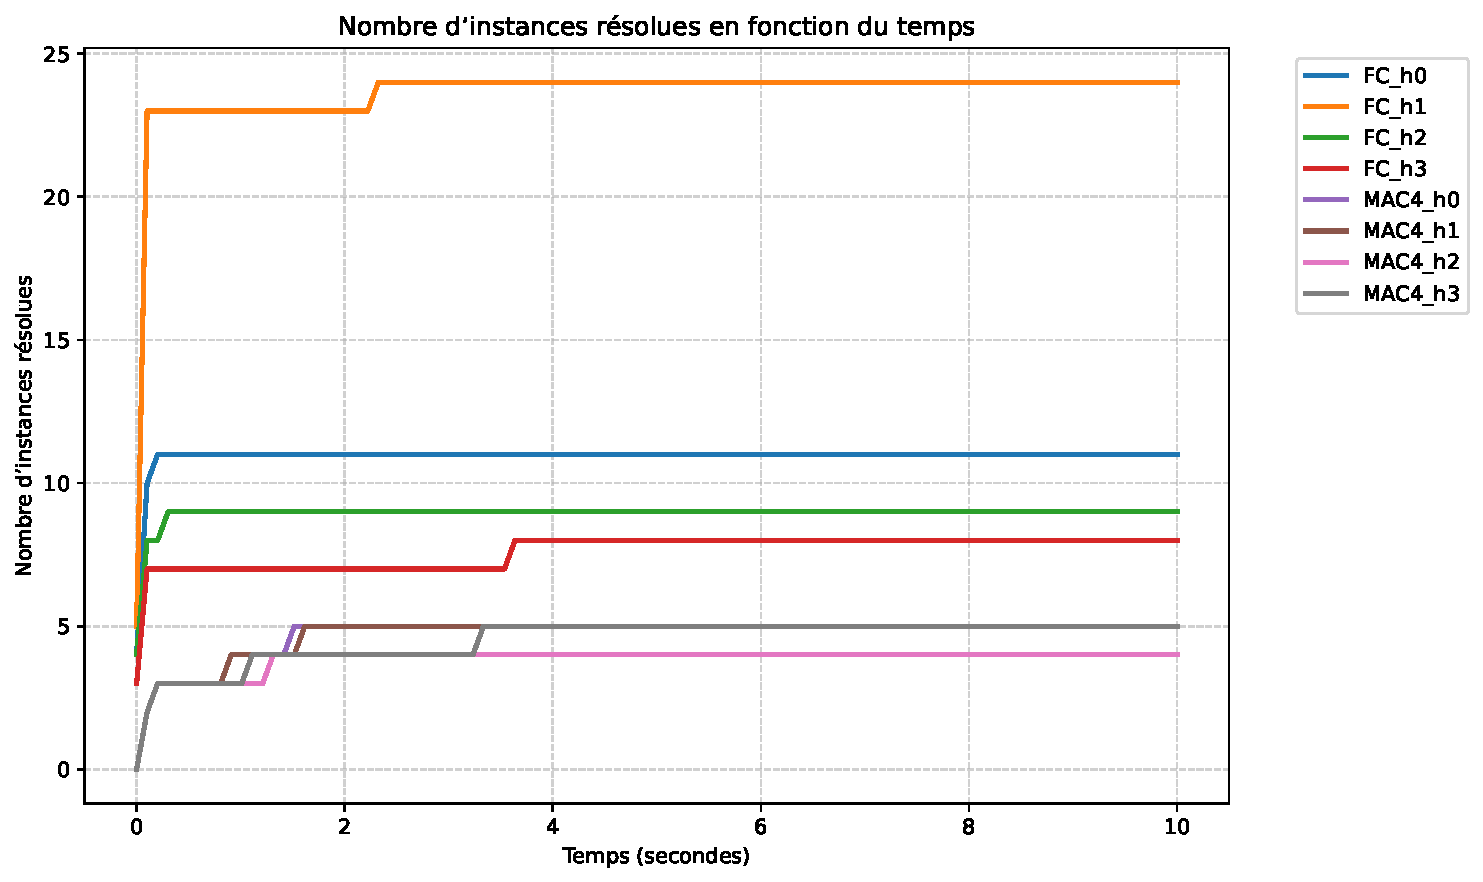
\includegraphics[width=1\textwidth]{Images/graph_coloring-h.pdf}
	\caption{Nombre d'instances de k-coloriage résolues par [FC] et [MAC] en fonction de l'heuristique de choix}
	\label{fig:coloriage-h}
\end{figure}

On maintient sur la figure \ref{fig:coloriage-h} les mêmes observations sur l'importance de l'heuristique de choix sur l'efficacité de nos algorithmes effectuées dans la partie précédente: [FC] demeure significativement plus performant que [MAC] avec une heuristique de choix identique mais un mauvais choix de variable peut suffisamment pénaliser un algorithme supposé efficace pour qu'il devienne moins bon qu'un autre avec une meilleure heuristique.

En se penchant plus spécifiquement sur les performances d'une heuristique de choix avec notre meilleur algorithme [FC], on observe:
\begin{itemize}
	\item \textbf{h2} est toujours une mauvaise heuristique de choix, ce qui est cohérent avec l'intuition que l'on peut s'en faire, en choisissant la variable la moins contrainte tôt dans notre recherche, on a plus de chances de tomber sur une instanciation infaisable et de devoir remonter haut dans l'arbre.
	\item \textbf{h0} demeure également moyenne, cette performance est uniquement due à la forme des instances qui nous sont données initialement, cette heuristique est celle qu'il faut réussir à vaincre ici avec les nouvelles introduites.
	\item L'heuristique aléatoire \textbf{h3} quant-à-elle perd en efficacité ici, elle se comporte moins bien que celle du plus grand domaine. Contrairement au problème des n-reines, où toutes les variables se contraignent deux-à-deux, dans le cas du coloriage, la matrice des contraintes est beaucoup plus éparse. Cela explique sans doute l'inefficacité du choix aléatoire des variables, car nous nous baladons alors dans le graphe initial indépendamment de sa structure de départ, qui est au cœur du problème.
	\item L'heuristique la plus efficace demeure \textbf{h1}, celle du plus petit domaine.
\end{itemize}

Nous observons que l'efficacité des différentes heuristiques de choix varie grandement en fonction de la structure du problème que l'on souhaite résoudre. Cela pourrait être une piste d'approfondissement de notre solveur.

\clearpage

\section{Conclusion}

Les bonnes performances obtenues sur le problème n-reines semblent indiquer que les choix de langage de programmation, structures de données, et d'implémentations étaient judicieux. En revanche, sur ce problème, la question de la représentation du problème s'est posée. En effet, le programme peut prendre jusqu'à quelques minutes pour charger en mémoire les instances les plus grandes. La représentation en extension atteint ici ses limites.\\

Le problème de k-coloriage s'est montré plus difficile sur les instances considérées, et on a pu constater une vraie sous-performance de notre moteur par rapport à des outils open-source plus matures, tel que le solveur open-source [CP-SAT] développé par Google. Pour améliorer les performances du moteur sur ce problème, on pourrait chercher à éliminer les solutions symétriques, et identifier des sous-structures expliquant une infaisabilité.\\

En ce qui concerne les méthodes utilisées, on peut conclure en évoquant les points suivants observés :

\begin{itemize}
	\item La méthode [FC] est celle qui a les meilleures performances sur l'ensemble des instances. C'est un bon compromis entre un simple backtrack, et une propagation complète des contraintes.
	\item Les méthodes [Bck] et [MAC4] ont en général de mauvaises performances, la première car elle ne permet pas d'élaguer suffisamment l'arbre de recherche, la seconde car la propagation des contraintes est, en pratique, trop lente.
	\item La méthode [MAC3] a des performances légèrement moins bonnes que [FC], mais bien meilleures que [MAC4]. En pratique, on préférera donc implémenter [AC3] que [AC4].\\
\end{itemize}


En ce qui concerne les heuristiques de choix de variables, on a pu constater que suivant les problèmes considérés, ce ne sont pas nécessairement les mêmes heuristiques qui donnent les meilleurs résultats en pratique. En particulier : 

\begin{itemize}
	\item L'heuristique de choix aléatoire de variable est préférable pour le problème n-reines.
	\item L'heuristique de choix de variable de plus petit domaine est préférable pour le problème de k-coloriage.
\end{itemize}

\end{document}
